\begin{figure}[H]
    \begin{subfigure}{0.25\linewidth}
        \centering
        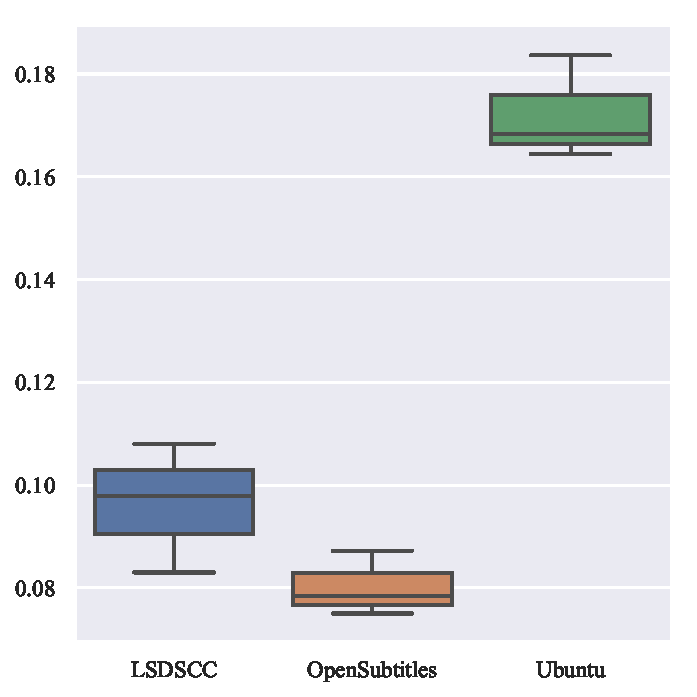
\includegraphics[width=\linewidth]{figure/boxplot/dataset/rouge_1/plot.pdf}
        \caption{ROUGE-1}
    \end{subfigure}%
    \begin{subfigure}{0.25\linewidth}
        \centering
        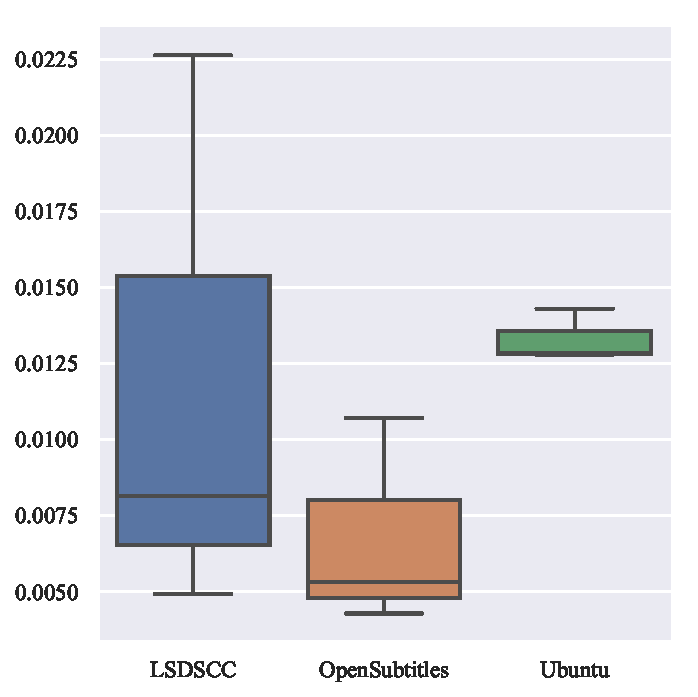
\includegraphics[width=\linewidth]{figure/boxplot/dataset/rouge_2/plot.pdf}
        \caption{ROUGE-2}
    \end{subfigure}%
    \begin{subfigure}{0.25\linewidth}
        \centering
        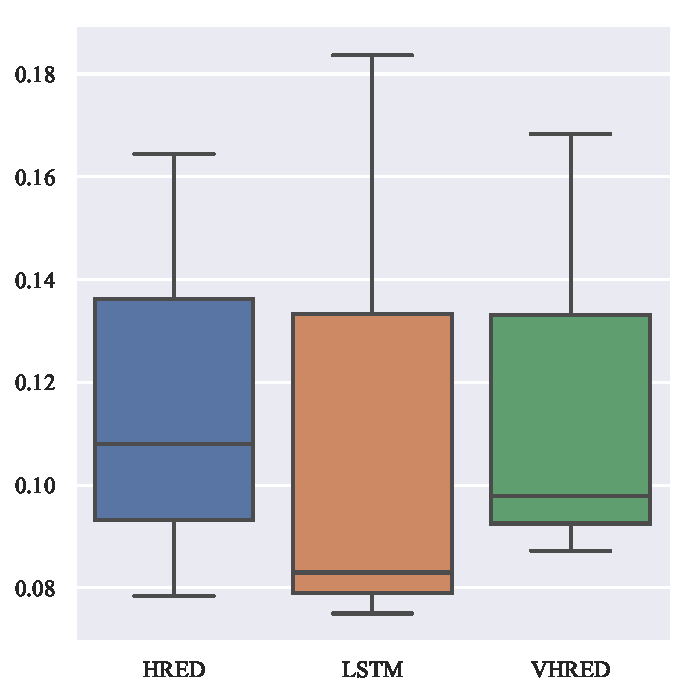
\includegraphics[width=\linewidth]{figure/boxplot/model/rouge_1/plot.pdf}
        \caption{ROUGE-1}
    \end{subfigure}%
    \begin{subfigure}{0.25\linewidth}
        \centering
        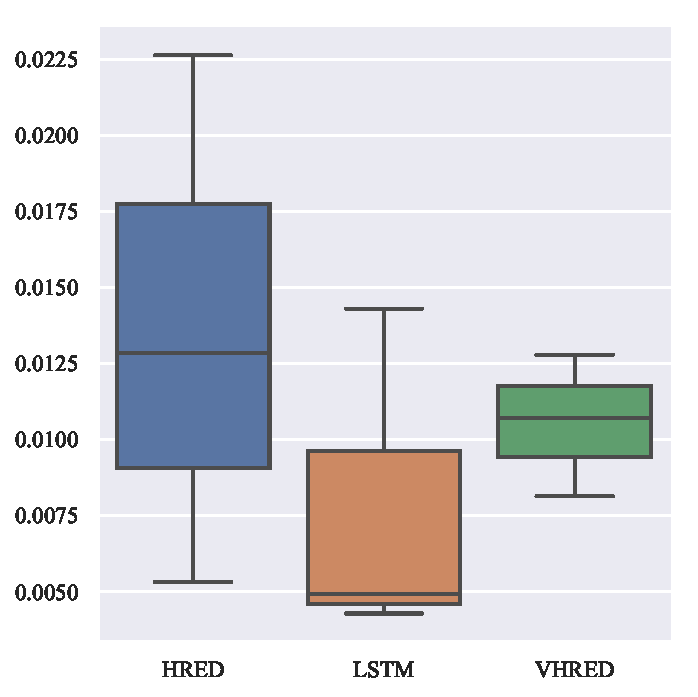
\includegraphics[width=\linewidth]{figure/boxplot/model/rouge_2/plot.pdf}
        \caption{ROUGE-2}
    \end{subfigure}
    \begin{subfigure}{0.25\linewidth}
        \centering
        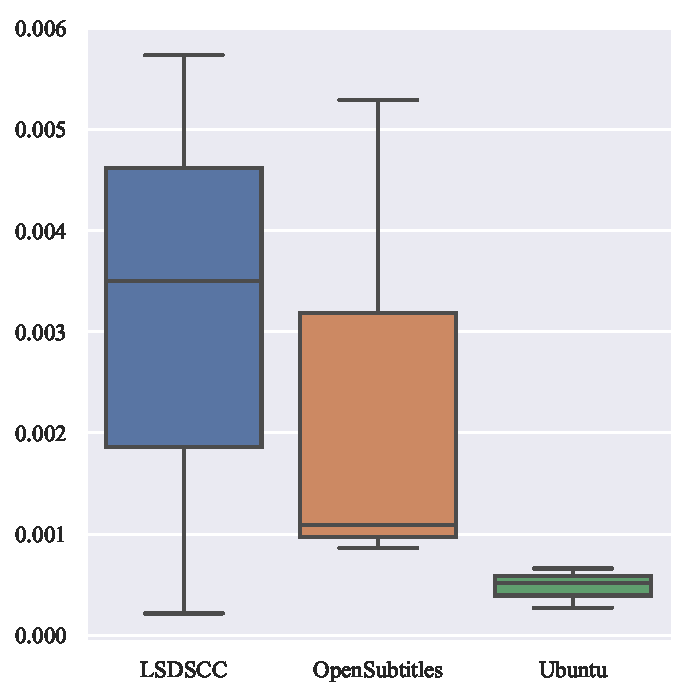
\includegraphics[width=\linewidth]{figure/boxplot/dataset/rouge_3/plot.pdf}
        \caption{ROUGE-3}
    \end{subfigure}%
    \begin{subfigure}{0.25\linewidth}
        \centering
        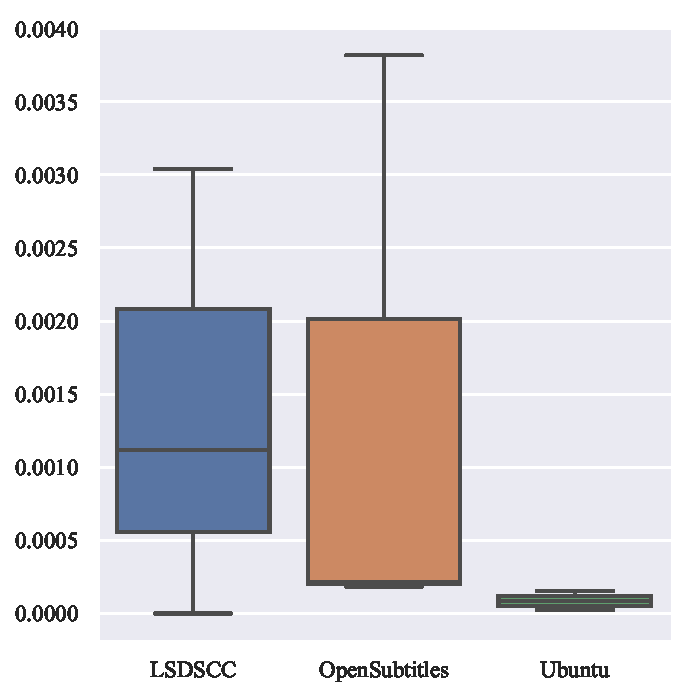
\includegraphics[width=\linewidth]{figure/boxplot/dataset/rouge_4/plot.pdf}
        \caption{ROUGE-4}
    \end{subfigure}%
    \begin{subfigure}{0.25\linewidth}
        \centering
        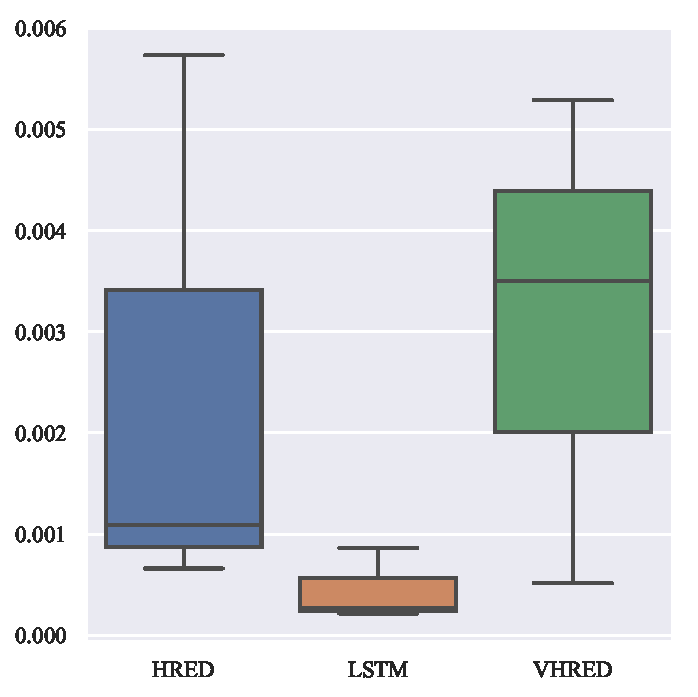
\includegraphics[width=\linewidth]{figure/boxplot/model/rouge_3/plot.pdf}
        \caption{ROUGE-3}
    \end{subfigure}%
    \begin{subfigure}{0.25\linewidth}
        \centering
        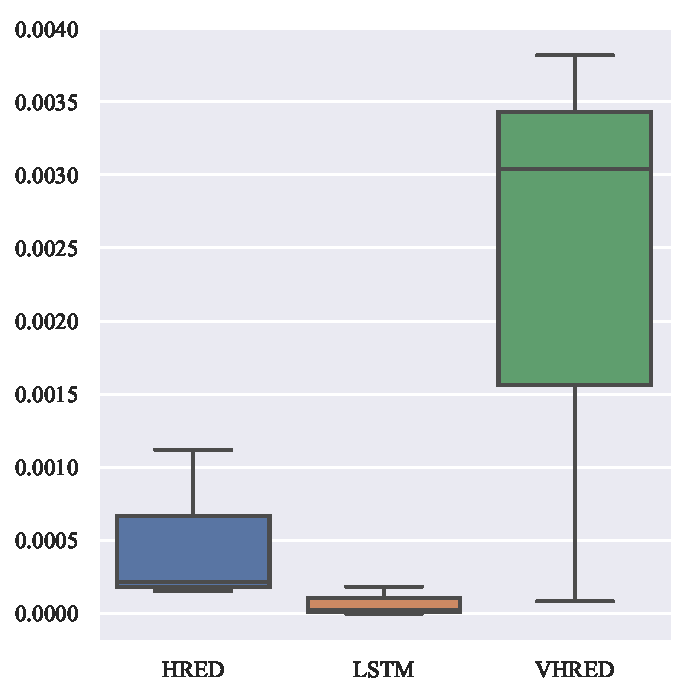
\includegraphics[width=\linewidth]{figure/boxplot/model/rouge_4/plot.pdf}
        \caption{ROUGE-4}
    \end{subfigure}
    \begin{subfigure}{0.25\linewidth}
        \centering
        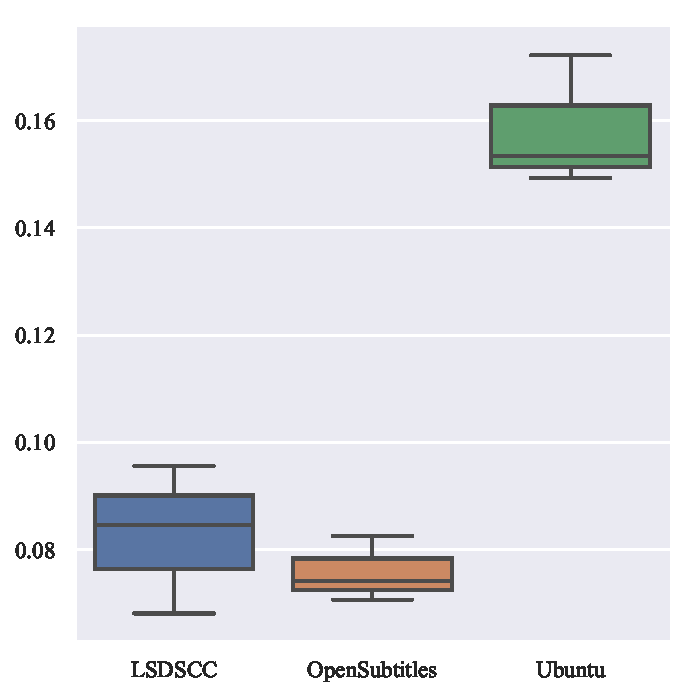
\includegraphics[width=\linewidth]{figure/boxplot/dataset/rouge_l/plot.pdf}
        \caption{ROUGE-L}
    \end{subfigure}%
    \begin{subfigure}{0.25\linewidth}
        \centering
        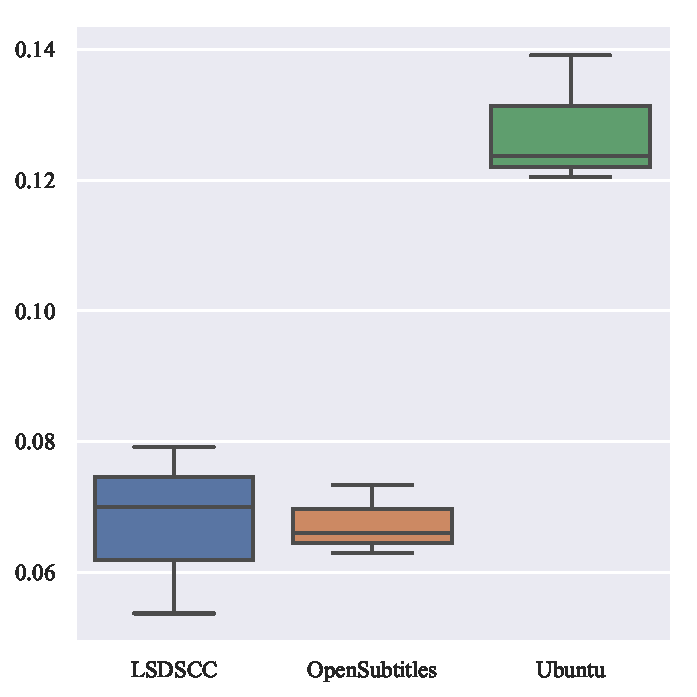
\includegraphics[width=\linewidth]{figure/boxplot/dataset/rouge_w/plot.pdf}
        \caption{ROUGE-W}
    \end{subfigure}%
    \begin{subfigure}{0.25\linewidth}
        \centering
        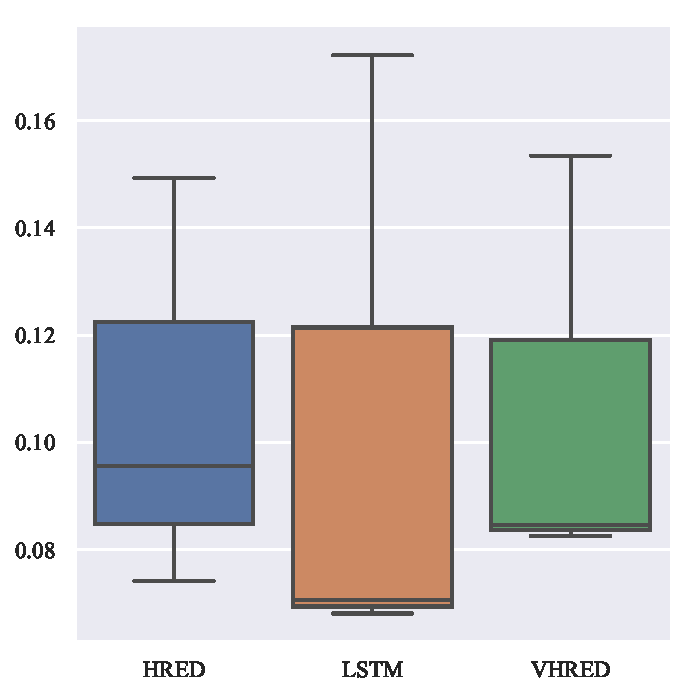
\includegraphics[width=\linewidth]{figure/boxplot/model/rouge_l/plot.pdf}
        \caption{ROUGE-L}
    \end{subfigure}%
    \begin{subfigure}{0.25\linewidth}
        \centering
        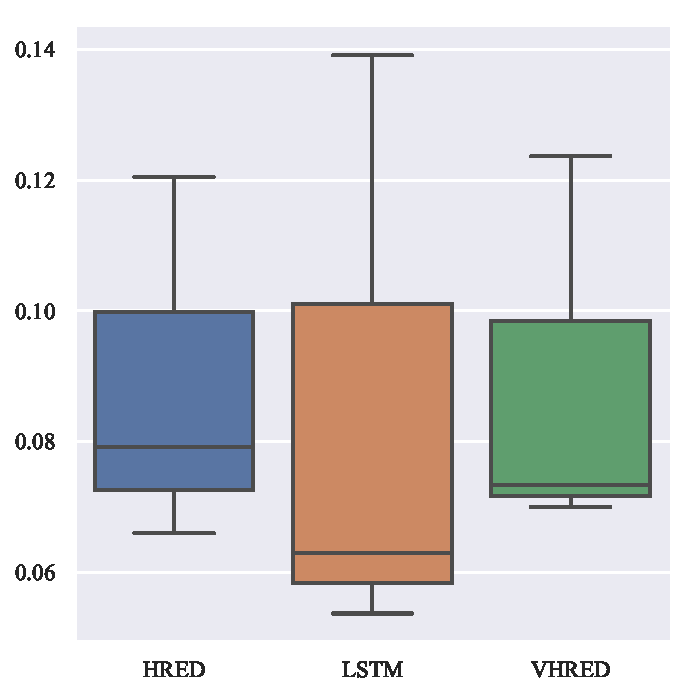
\includegraphics[width=\linewidth]{figure/boxplot/model/rouge_w/plot.pdf}
        \caption{ROUGE-W}
    \end{subfigure}
    \centering
    \caption{不同数据集上的ROUGE分布(左),不同模型的ROUGE分布(右)}
    \label{fig:ROUGE_dataset}
\end{figure}
